\newpage
\hypertarget{treeToModel tex}{}
\subsection{Tree To model text source}
\texHeader

Plan : separate the transformation into smaller, modular steps. So we've established one correspondence type. First: Transform the
parent \texttt{myLibrary} \texttt{Folder} into a \texttt{Library}. Then we want to establish every subfolder as a \texttt{Shelf} (i.e., separate shelves
for English and French). Finally, we then want to translate the dictionary file trees which have a defined \texttt{title}, \texttt{author}, and \texttt{content}
node. The setup of rules and other TGG elements are explained in detail in Part IV.

\begin{itemize}
\subsubsection{FolderToLibraryRule} % ---------------------------------

\item[$\blacktriangleright$] Expand \texttt{DictionaryCodeAdapter}, right-click on \texttt{Rules}, and navigate to ``New / TGG Rule." Name it
\texttt{Folder\-To\-Lib\-rary\-Rule}.

\item[$\blacktriangleright$] This is a simple rule. All we'll need to do is create folder and library object variables, create a correspondence link between
them so that they always remain consistent with one another, and create a single constraint equating the \texttt{name} of the folder to the \texttt{name} of the
library. Build your rule until it resembles Fig.~\ref{eclipse:FolderToLibraryRule}.

\begin{figure}[htbp]
\begin{center}
  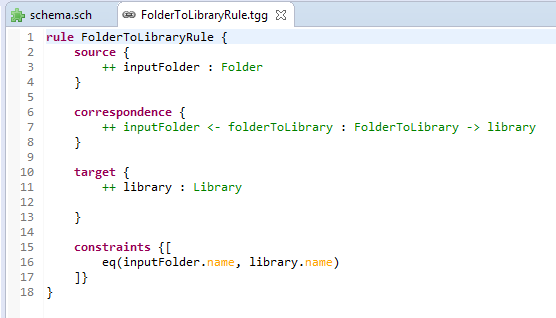
\includegraphics[width=\textwidth]{eclipse_FolderToLibraryRule}
  \caption{The TGG transformation will begin with this rule.}
  \label{eclipse:FolderToLibraryRule}
\end{center}
\end{figure}

\item[$\blacktriangleright$] Did you notice that every element in this rule is green? This is the starting point for the transformation, where this rule must
guarantee that, in either direction, \texttt{Folder} and \texttt{Library} instances exist upon exit. To see this rule modeled in the visual syntax, check out
Fig.~\ref{ea:FolderToLibraryRule}.

\subsubsection{ForAllShelfRule} % ---------------------------------

\item[$\blacktriangleright$] Let's use the context from the previous rule and create the \texttt{ForAllShelfRule} as described in 
Fig.~\ref{eclipse:ForAllShelvesRule}. Don't forget to add the new \texttt{FolderToShelf} correspondence type to \texttt{schema.sch} 
(Fig.~\ref{eclipse:updatedSchema}).

\vspace{0.5cm}

\begin{figure}[htbp]
\begin{center}
  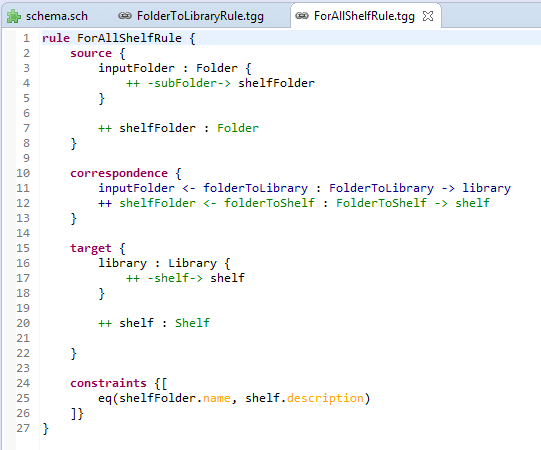
\includegraphics[width=0.9\textwidth]{eclipse_ForAllShelfRule}
  \caption{ForAllShelfRule complete}
  \label{eclipse:ForAllShelvesRule}
\end{center}
\end{figure}

\begin{figure}[htbp]
\begin{center}
  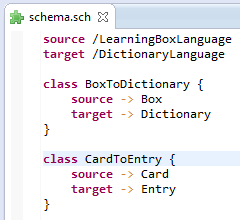
\includegraphics[width=0.7\textwidth]{eclipse_updatedSchema}
  \caption{Update the TGG Schema with all new correspondence types}
  \label{eclipse:updatedSchema}
\end{center}
\end{figure}

\item[$\blacktriangleright$] The driving reason why this rule is independent, and not included with our intializing rule is simply because we don't know how
many subfolders the input library folder will have. By separating it, this rule may be invoked (in the forward direction) whenever a new folder and
\texttt{subFolder} reference are matched to \texttt{inputFolder}. It will then create a new \texttt{shelf}, updating the appropriate reference in
\texttt{library}.

\vspace{0.5cm}

Now for the meatiest part of our transformation, transforming each dictionary \texttt{File} into a dictionary instance. Reviewing \texttt{tree.xmi}
(Fig.~\ref{eclipse:treeResult}), you'll notice that each \texttt{.dictionary} file is turned into a parent \texttt{DICTIONARY} node with at least three children
- one node for the \texttt{title} of the dictionary, one for the \texttt{email} of the author, and one \texttt{ENTRY} node per entry as listed in the source
files. What needs to be separated? What elements do we know will always exist? 

\newpage

We know we'll always have a title node, but we're not sure if an author will be included, and we won't know how many entires are involved. Therefore, one
should actually create at least three different rules to handle this step of the transformation. Let's build the primary rule that will match to every
\texttt{.dictionary} file first.

\subsubsection{NodeToDictionaryRule} % ---------------------------------

\item[$\blacktriangleright$] Create a rule name \texttt{NodeToDictionaryRule}, and build it as indicated in Fig.~\ref{eclipse:NodeToDictionaryRule}.

\begin{figure}[htbp]
\begin{center}
  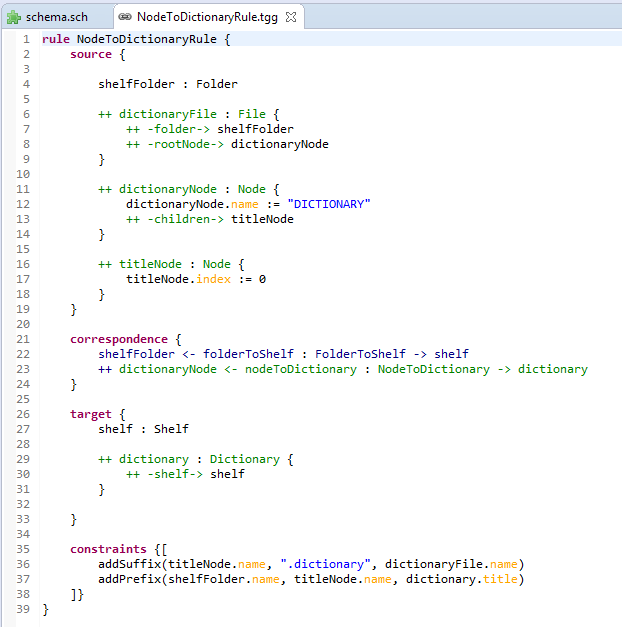
\includegraphics[width=\textwidth]{eclipse_NodeToDictionaryRule}
  \caption{NodeToDictionary complete}
  \label{eclipse:NodeToDictionaryRule}
\end{center}
\end{figure}

\item[$\blacktriangleright$] As you can see, this rule demands that a \texttt{shelfFolder} and \texttt{shelf} already exist before executing, implying that this
rule can only be called after executing \texttt{ForAllShelfRule}. An attribute constraint is used with \texttt{titleNode} to ensure that the correct child
\texttt{Node} is matched to \texttt{dictionaryNode} (and not accidentally an author or entry node).

\item[$\blacktriangleright$] This rule also imposes two constraints, one for each direction. In the forward transformation, we want to add the name of
the shelf to the dictionary file's title (i.e., ``english'' and ``numbers1-10'') and set it as the target's \texttt{name}. Though this may be somewhat abstract
at first, imagine this constraint is actually called ``add/remove Suffix'' since, during the inverse transformation, this constraint also will ensure the name
of the shelf is not present.

\item[$\blacktriangleright$] Similarly, in the backwards transformation, the transformation needs to generate a valid \texttt{dictionaryFile} name, and it does
so by appending \texttt{.dictionary} to the end of \texttt{titleNode.name}.

\newpage

\subsubsection{ForAllEntryRule} % ---------------------------------

\item[$\blacktriangleright$] Let's handle the \texttt{Entry} elements next. We want to demand the \texttt{Node\-To\-Dict\-ion\-ary\-Rule} to execute first so
that we can assume the \texttt{dictionaryNode} context informatione exists. Create \texttt{ForAllEntryRule}, and build it so it matches
Fig.~\ref{eclipse:ForAllEntryRule}.

\begin{figure}[htbp]
\begin{center}
  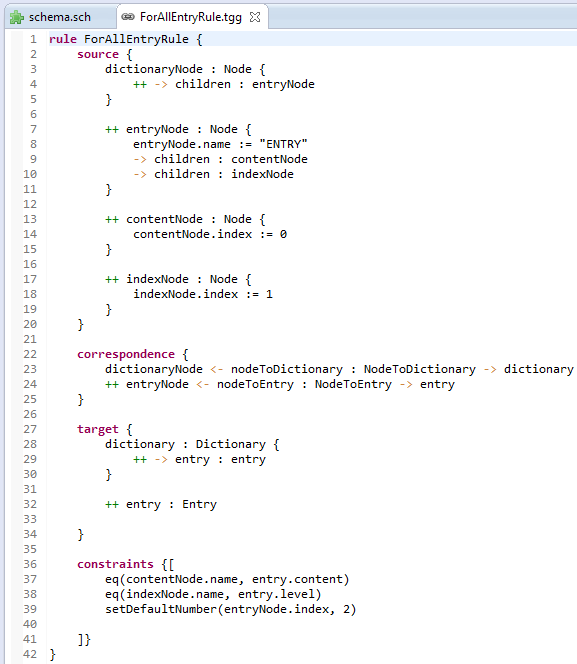
\includegraphics[width=0.9\textwidth]{eclipse_ForAllEntryRule}
  \caption{ForAllEntry complete}
  \label{eclipse:ForAllEntryRule}
\end{center}
\end{figure}

\item[$\blacktriangleright$] Each \texttt{entryNode} has two child elements, one to store its index value in \texttt{dictionaryNode}'s collection of nodes, and
one to store its actual keyword and definition data. Similar to \texttt{indexNode}, both of these childs must be bound so that the constraints are able to match
the correct data to the target \texttt{entry}. We don't need an attribute constraint on \texttt{entryNode} as \texttt{titleNode} is already bound to 0, and
later \texttt{authorNode} will be bound to 1. This set up will then assume any other index value (i.e., indices >=2) is an \texttt{entry}, which is exactly what
we want.

\newpage

\subsubsection{ForAllNewAuthorRule} % ---------------------------------

Now to handle \texttt{author}s. Transforming forwards from a \texttt{authorNode} to an \texttt{author} isn't as simple as an
\texttt{entryNode}, where you create an \texttt{entry} every time you find a valid match. Instead, we have to account for the possiblity of multiple authors in
a single \texttt{library}, as noticed with the first two dictionary files in ``french.'' While some users may not care, why not provide handling for the case
where a user doesn't care about multiple instances of authors (a one-to-one ratio), and one case where a user wants to optimize their target with one library
instance for each unique \texttt{authorNode}. For \texttt{contact@pons.de}, this means there can only be one instance of \texttt{authorNode} with a single
\texttt{library} reference to \texttt{Library}, but two \texttt{dictionary} references to both number dictionaries.

\item[$\blacktriangleright$] Create \texttt{ForAllNewAuthorRule}, and complete it as depicted in Fig.~\ref{eclipse:ForAllNewAuthorRule}. You can see that for
every \texttt{authorNode} instance it's able to find, it creates an \texttt{author}.

\begin{figure}[htbp]
\begin{center}
  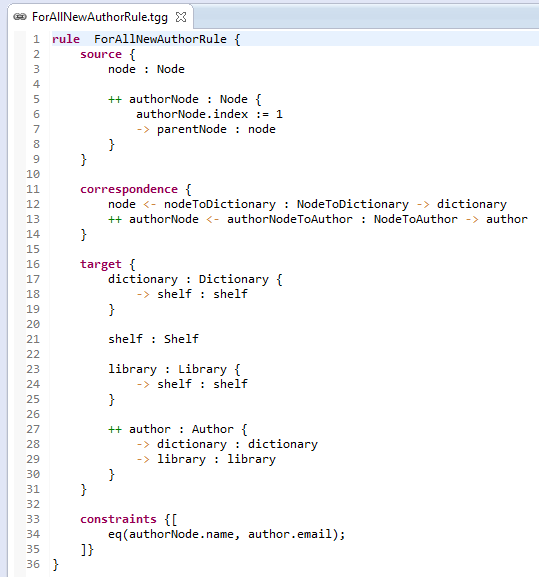
\includegraphics[width=\textwidth]{eclipse_ForAllNewAuthorRule}
  \caption{ForAllAuthor complete}
  \label{eclipse:ForAllNewAuthorRule}
\end{center}
\end{figure}

\subsubsection{ExistingAuthorRule} % ---------------------------------

\item[$\blacktriangleright$] Similarly, create \texttt{ForExistingAuthorRule} as specified in Fig.~\ref{eclipse:ForExistingAuthorRule}. You should be able to
copy and paste the majority of the previous rule. In fact, the only thing you need to change are two small characters in front of \texttt{author} and its
\texttt{dictionary} reference, forcing the rule to assume and match to some context \texttt{author}, but still create a new link between the current dictionary
file and previous author.

\begin{figure}[htbp]
\begin{center}
  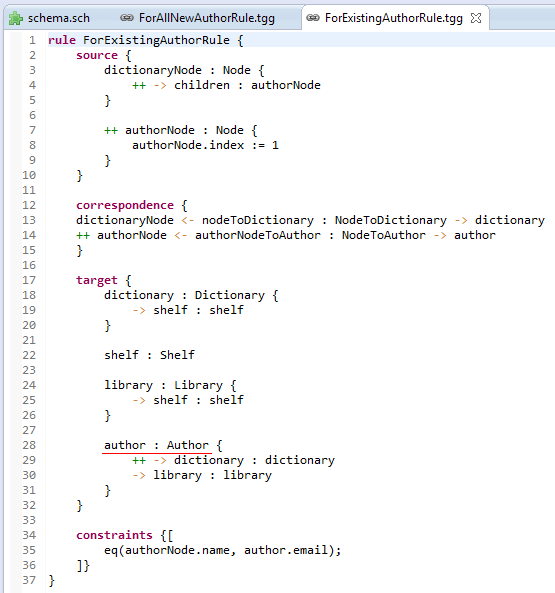
\includegraphics[width=\textwidth]{eclipse_ForExistingAuthorRule}
  \caption{ForExistingAuthor complete}
  \label{eclipse:ForExistingAuthorRule}
\end{center}
\end{figure}

\newpage

\item[$\blacktriangleright$] Great work! You have now specified six different rules (with a focus on the forward direction) to perform a text-to-model
transformation! For confirmation, your final schema and package explorer should now resemble Fig.~\ref{eclipse:schemaFinal}.

\vspace{0.5cm}

\begin{figure}[htbp]
\begin{center}
  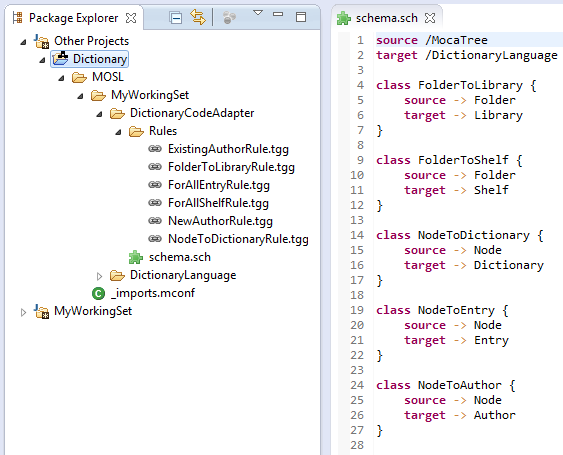
\includegraphics[width=\textwidth]{eclipse_finalSchema}
  \caption{Final schema}
  \label{eclipse:schemaFinal}
\end{center}
\end{figure}

\vspace{0.5cm}

\item[$\blacktriangleright$] Given that everything has been done correctly, and MOSL hasn't reported any errors when you saved everything, build your TGG! If
there are problems, be sure to double check for spelling or character symbols. 

\end{itemize}
